\chapter{Results\label{cha:chapter6}}
\section{Data Acquisition}
The data acquisition was performed with 27 subjects in total, 12 (44\%) females and 15 (56\%) males. Participants had an average age of 26.4 years (17, 53, 6.39) and all 27 were right-handed (100\%). 19 (70\%) were students, 8 (30\%) had other occupations.
18 (66\%) subjects stated that their most used input modality is the their thumb while 4 (14\%) preferred using their index finger and 5(18\%) use both thumbs during interactions.\\

\begin{figure}[h!]
  \centering
  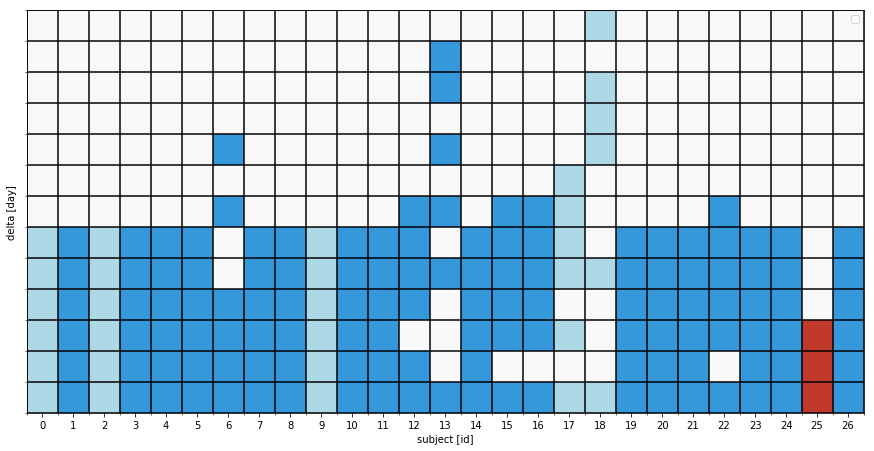
\includegraphics[width=1\textwidth]{participation_push.png}
  \caption{The figure shows on which days the participants took part in the field study. Light blue subjects which did not receive push notifications while subjects with dark blue marks had received push notifications. Red rectangles indicates a dropped out subject.} \label{fig:participation}
\end{figure}

In regards to the participation during the study, 26 subjects managed to finish all laboratory and field study trials while 1 subject dropped out in the field study. Figure \ref{fig:participation} shows on which day individual participants performed trails. 4 participants did not accept push notification and were therefore not reminded on a daily basis.

In total over 46.000 taps were generated in the whole data acquisition phase. To be more precise, approx. 25.000 taps were collected on the 5x4 grid, over 15.000 taps on the 4x3 grid and more than 5.000 taps on the 2x2 grid. Concerning the distribution of the body posture and the input modality, subjects used their thumb more frequently compared to the index finger and sat more often during the trails compared to the standing posture. The distributions are illustrated in figure \ref{fig:bpimdis}.

The devices used to obtain the tap information were 12 (45\%) Apple iPhone 6s, 10 (37\%) iPhone 6 and the least common device was the iPhone 7 with 5 (18\%).

In order to visualize the data collected, a t-Distributed Stochastic Neighbor Embedding (t-SNE) embedding is shown in figure \ref{fig:tsne} where the 230-dimensional feature vector has been reduced to 2 dimensions. Furthermore, a plot showing the interpolated gyroscope and accelerometer signals acquired during a single tap generation trial is to be found in the Appendix.

\begin{figure}
  \centering
  \begin{tabular}{cc}
    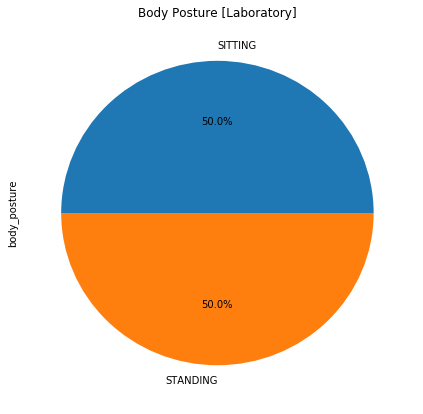
\includegraphics[width=50mm]{results/pie-bp-lab} &   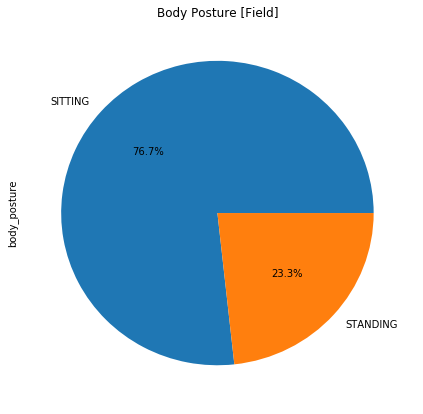
\includegraphics[width=50mm]{results/pie-bp-field} \\
   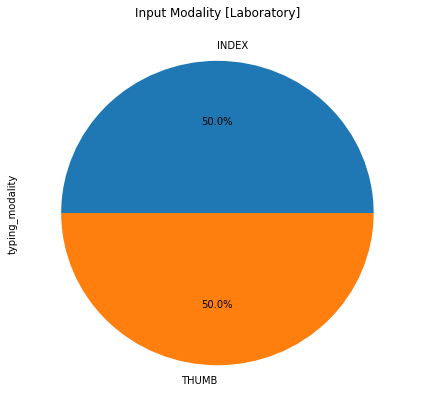
\includegraphics[width=50mm]{results/pie-im-lab} &   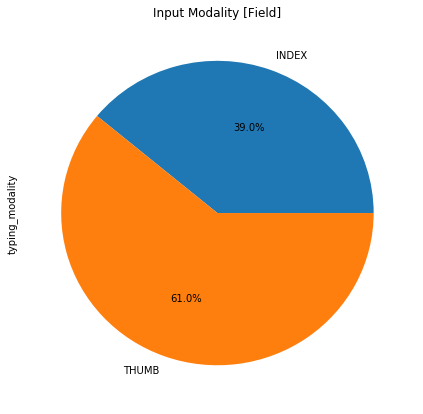
\includegraphics[width=50mm]{results/pie-im-field} \\
  \end{tabular}
  \caption{The pie charts show the distribution of the input modalities and the body postures used in the field and the laboratory trials.}\label{fig:bpimdis}
\end{figure}


\afterpage{%
\begin{figure}
  \centering
  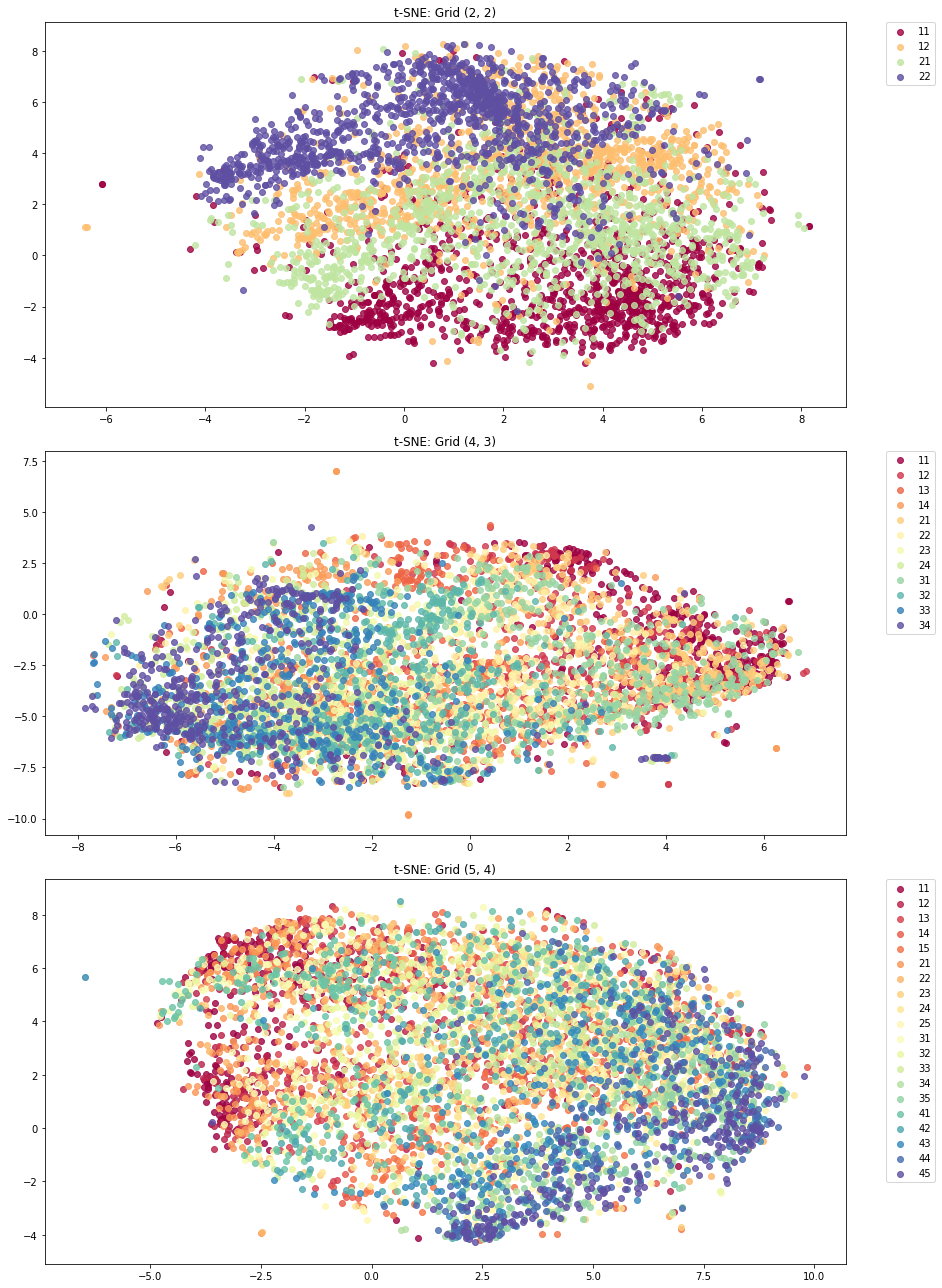
\includegraphics[width=0.9\textwidth]{results/tsne_2.png}
  \caption{ Visualization of 230-dimensional feature vectors reduced to 2 dimensions.
  The used t-SNE dimensionality reduction technique is unsupervised, thus it does
  not consider the labels during the optimization} \label{fig:tsne}
\end{figure}
\clearpage
}

\section{Laboratory and Field Comparison}
For the analysis between the controlled and the uncontrolled environment, a subset of the overall training material has been filtered based on the environment, grid size and the mobile device. After performing a grid search of the hyperparameter space for the SVM and, likewise, for the ANN, a 10-fold cross validation has been performed on the best of the two estimators yielding the highest mean accuracy.

\subsubsection{2x2 Grid}

\begin{figure}[h!]
  \centering
  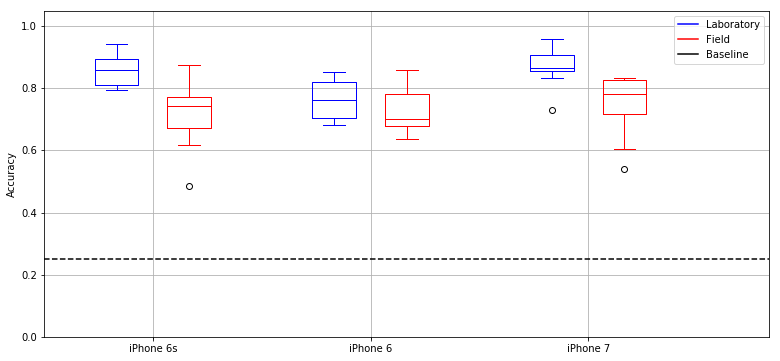
\includegraphics[width=1\textwidth]{results/lab-vs-field-2x2.png}
  \caption{The figure shows the tap inference accuracies for the 2x2 grid of the 10-fold cross-validation. The measured classification accuracies are above the guessing probability of $\frac{1}{4} = 25\%$.} \label{fig:lab2x2}
\end{figure}

For the 2x2 grid, the results show mean accuracy measures in range 0.79 to 0.87 for the laboratory environment and ranges 0.68 to 0.76 for the field environment. Furthermore, the iPhone 7 data scores highest with a mean accuracy score of the 0.85 for this particular classification problem.

\begin{table}[h!]
  \centering
  \begin{tabular}{|l|l|c|c|c|c|c|}
    \cline{3-6}
    \multicolumn{2}{c}{} & \multicolumn{4}{|c|}{\textbf{Accuracy}}  \\
    \hline
    \textbf{Device} & \textbf{Environment} & mean &   min &   max  & std &  \textbf{Classifier} \\
    \hline
    iPhone 6 & Laboratory &      0.79 &     0.72 &     0.87 &     0.05 &  SVM \\
    & Field &      0.71 &     0.62 &     0.83 &     0.06 &  SVM \\
    \hline
iPhone 6s     & Laboratory &      0.85 &     0.77 &     0.96 &     0.06 &  SVM \\
& Field &      0.68 &     0.52 &     0.81 &     0.09 &  SVM \\
    \hline
iPhone 7 & Laboratory &      0.87 &     0.73 &     0.96 &     0.08 &  SVM \\
& Field &      0.76 &     0.56 &     0.92 &     0.09 &  SVM \\
    \hline
  \end{tabular}
  \caption{Classification results for the 2x2 tapping grid. Notably, the SVM outperforms the ANN for this task.}
\end{table}

% Results show that the model trained with data from the iPhone 7 outperform the models trained with the iPhone 6 and iPhone 6s, respectively. The iPhone 6 models shows least accuracy scores of 0.76 (+/- 0.06) for the controlled and 0.73 (+/- 0.07) for the uncontrolled environment.

% For the comparison of devices, the results yield that the iPhone 7 scores higher accuracies compared to the iPhone 6 and and the iPhone 6s for both environments. The iPhone 6 scores lowest with a mean accuracy of 0.76 (+/- 0.85) while the iPhone 7 performs best with a mean accuracy of 0.87 (+/- 0.96) in the controlled environment. For the field environnement the iPhone 7 scores a mean accuracy of 0.75 (+/- 0.83) while the iPhone 6 shows 0.73 (+/- 0.86).

Moreover, across all devices, the results list that the mean accuracies for the field data are always lower compared to the laboratory data. The fact that the classification measures for both environments differ significantly is confirmed by a Wilcoxon signed-rank test yielding that the fold accuracies in the laboratory were significantly higher than the fold accuracies in the field environment Z = 5, p < 0.05.

\subsubsection{4x3 Grid}

For the 4x3 grid, the analysis shows mean accuracy scores in range 0.46 to 0.59 for the laboratory environment and ranges 0.40 to 0.47 for the field environment. Furthermore, the iPhone 7 data scores highest with a mean accuracy score of the 0.59 for this 12-class problem.

\begin{figure}[h!]
  \centering
  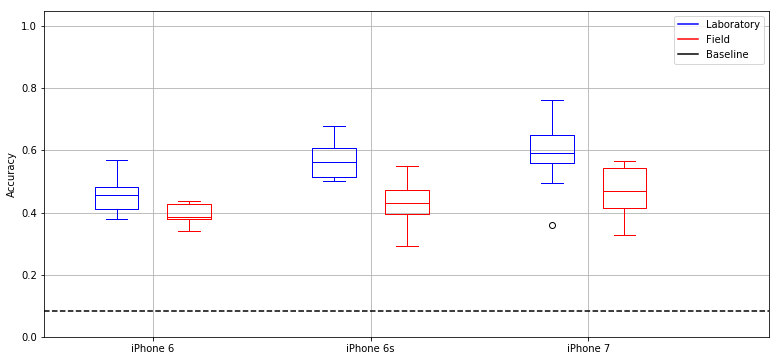
\includegraphics[width=1\textwidth]{results/lab-vs-field-4x3.png}
  \caption{The figure shows the tap inference accuracies for the 4x3 grid of the 10-fold cross-validation. The measured inference accuracies are above the probability baseline of guessing ($\frac{1}{12}= 8.33\%$ for the 12 distinguishable buttons).} \label{fig:participation}
\end{figure}

\begin{table}[h!]
  \centering
\begin{tabular}{|l|l|c|c|c|c|c|}
  \cline{3-6}
  \multicolumn{2}{c}{} & \multicolumn{4}{|c|}{\textbf{Accuracy}}  \\
  \hline
  \textbf{Device} & \textbf{Environment} & mean &   min &   max  & std &  \textbf{Classifier} \\
  \hline
  iPhone 6 & Laboratory &      0.46 &     0.38 &     0.57 &     0.06 &  SVM \\
  & Field &      0.40 &     0.34 &     0.44 &     0.03 &  SVM \\
  \hline
iPhone 6s  & Laboratory &      0.57 &     0.50 &     0.68 &     0.06 &  SVM \\
 &   Field    &      0.43 &     0.29 &     0.55 &     0.07 &  ANN \\
 \hline
iPhone 7   & Laboratory &      0.59 &     0.36 &     0.76 &     0.11 &  SVM \\
& Field &      0.47 &     0.33 &     0.57 &     0.08 &  SVM \\
  \hline
\end{tabular}
  \caption{Classification results for the 4x3 tapping grid.}
\end{table}

A performed Wilcoxon signed-rank test shows that the classification results for both environments differ significantly. The fold accuracies in the laboratory were statistically higher than the fold accuracies in the field environment Z = 19, p < 0.05.

\subsubsection{5x4 Grid}
For the grid with 20 distinguishable areas the inference accuracies measures range from 0.35 to 0.43 for the laboratory and 0.28 to 0.32 for the field data, respectively. Aligning with the previous results, the iPhone 7 shows highest mean accuracy scores of 0.43 for the data collected in the laboratory. 

\begin{figure}[h!]
  \centering
  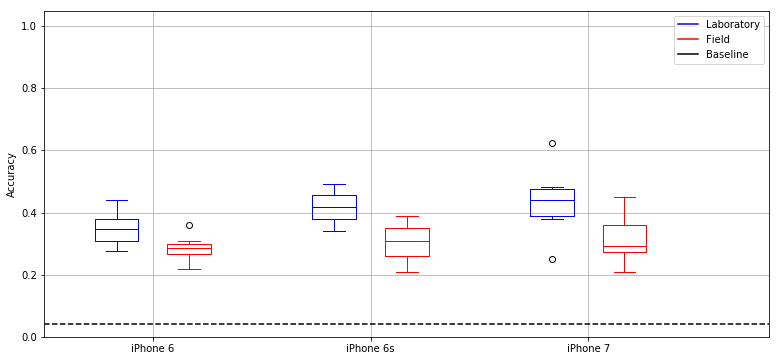
\includegraphics[width=1\textwidth]{results/lab-vs-field-5x4.png}
  \caption{The figure shows the tap inference accuracies for the 5x4 grid of the 10-fold cross-validation. Results show that all inference accuracies are above the baseline of $\frac{1}{20} = 5\%$ for this classification problem.} \label{fig:results-lf-5x4}
\end{figure}

% For the 4x3 grid, the analysis shows mean accuracy scores in range 0.46 to 0.59 for the laboratory environment and ranges 0.40 to 0.47 for the field environment. Furthermore, the iPhone 7 data scores highest with a mean accuracy score of the 0.59 for this 12-class problem.

% For the grid with 20 distinguishable buttons the inference accuracies range from 0.46 (+/- 0.11) on the iPhone 7 to 0.28 (+- 0.03) for the iPhone 6. 

Furthermore, The Wilcoxon signed-rank test shows that the classification results for both environments alter significantly. The fold accuracies in the laboratory were significantly higher than the fold accuracies in the field environment Z = 12, p < 0.05.

\begin{table}[h!]
  \centering
  \begin{tabular}{|l|l|c|c|c|c|c|}
    \cline{3-6}
    \multicolumn{2}{c}{} & \multicolumn{4}{|c|}{\textbf{Accuracy}}  \\
    \hline
    \textbf{Device} & \textbf{Environment} & mean &   min &   max  & std &  \textbf{Classifier} \\
    \hline
    iPhone 6 & Lab &      0.35 &     0.28 &     0.44 &     0.05 &  ANN \\
    & Field &      0.28 &     0.22 &     0.36 &     0.04 &  ANN \\
    \hline
    iPhone 6s & Lab &      0.42 &     0.34 &     0.49 &     0.05 &  SVM \\
    &   Field    &    0.31 &     0.21 &     0.39 &     0.06 &  ANN \\
    \hline
    iPhone 7 & Lab &      0.43 &     0.25 &     0.62 &     0.09 &  SVM \\
    & Field &      0.32 &     0.21 &     0.45 &     0.08 &  SVM \\    
    \hline
  \end{tabular}
  \caption{Classification results for the 5x4 tapping grid.}
\end{table}


\section{Input Modalities Comparison}
As for the comparison between controlled and uncontrolled environments, the same classification experiment was performed to detect differences in the predictive models between the two input modalities: Index finger and thumb. As subjects were free to decide which input modality to use during the field study, the sample size has been adjusted in order to train each classifier with the same amount of training material.

Classifier trained for the individual grid sizes show similar results. For this reason, only the results for the 5x4 grid will be shown here. The results for the other grid sizes are listed in the Appendix.

\begin{figure}[h!]
  \centering
  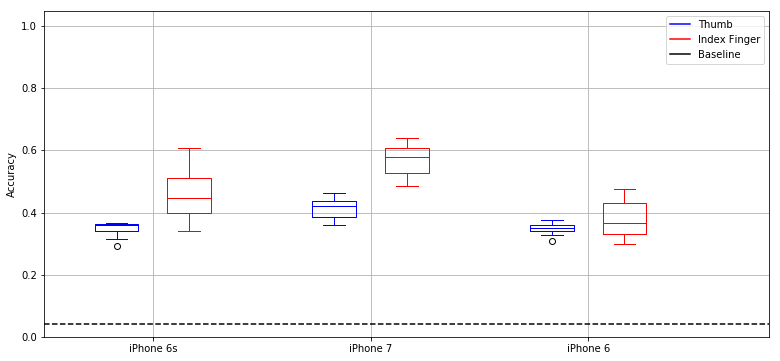
\includegraphics[width=1\textwidth]{results/index-vs-thumb-5x4.png}
  \caption{The figure shows the tap inference accuracies for the 5x4 grid of the 10-fold cross-validation.} \label{fig:participation}
\end{figure}

For the 5x4 grid, the results show that across all devices the mean inference accuracies for estimators trained with the thumb taps were lower compared to the classifiers trained with data containing index finger taps. For the iPhone 7, the estimator yields a mean accuracy of 0.54 for index finger samples compared to 0.38 for data representing the thumb as input modality. The same results apply for the other tested devices. A Wilcoxon signed-rank test shows that the classification results for both input modalities differ significantly. The fold accuracies on thumb data were statistically lower than the fold accuracies on index finger data Z = 29, p < 0.05.


\begin{table}[h!]
  \centering
\begin{tabular}{|l|l|c|c|c|c|c|}
  \cline{3-6}
  \multicolumn{2}{c}{} & \multicolumn{4}{|c|}{\textbf{Accuracy}}  \\
  \hline
  \textbf{Device} & \textbf{Input Modality} & mean &   min &   max  & std &  \textbf{Classifier} \\
  \hline
  iPhone 6 & Index &      0.38 &     0.28 &     0.47 &     0.06 &  ANN \\
  & Thumb &      0.35 &     0.33 &     0.37 &     0.01 &  ANN \\
  \hline
iPhone 6s & Index &      0.44 &     0.35 &     0.54 &     0.06 &  SVM \\
  & Thumb &      0.37 &     0.33 &     0.41 &     0.02 &  ANN \\
  \hline
  iPhone 7 & Index &      0.54 &     0.45 &     0.59 &     0.04 &  SVM \\
  & Thumb &      0.38 &     0.30 &     0.42 &     0.04 &  ANN \\
  \hline
\end{tabular}
  \caption{Classification results for the 5x4 tapping grid for both input modalities: thumb and index finger.}
\end{table}

\section{Body Posture Comparison}
For the comparison between the two body postures (sitting and standing) the overall training material was filtered based on the device and body posture the user had while tapping. Furthermore, only index finger taps are considered in this experiment. As for the comparison of input modalities, the amount of training material was balanced.

\begin{table}[h!]
  \centering
\begin{tabular}{|l|l|c|c|c|c|c|}
  \cline{3-6}
  \multicolumn{2}{c}{} & \multicolumn{4}{|c|}{\textbf{Accuracy}}  \\
  \hline
  \textbf{Device} & \textbf{Input Modality} & mean &   min &   max  & std &  \textbf{Classifier} \\
  \hline
  iPhone 6 & Standing &      0.30 &     0.19 &     0.45 &     0.08 &  SVM \\
  & Sitting &      0.35 &     0.29 &     0.41 &     0.03 &  ANN \\
  \hline
iPhone 6s   & Standing &      0.37 &     0.34 &     0.42 &     0.03 &  SVM \\
& Sitting &      0.47 &     0.34 &     0.61 &     0.08 &  SVM \\
  \hline
  iPhone 7 &    Sitting     &      0.58 &     0.44 &     0.82 &     0.11 &  SVM\\
  & Standing &      0.43 &     0.35 &     0.52 &     0.05 &  ANN \\
  \hline
\end{tabular}
  \caption{Classification results for the 5x4 tapping grid for both body postures: sitting and standing.}
\end{table}

Only the 5x4 grid is presented here, as similar results are found for the other grid sizes (see Appendix). The findings show that the mean accuracies between the two body modalities differ (See figure \ref{fig:bodypos5x4}). This is also indicated in a Wilcoxon signed-rank test showing that the classification results for both factors differed significantly Z = 31, p > 0.05.

\begin{figure}[h!]
  \centering
  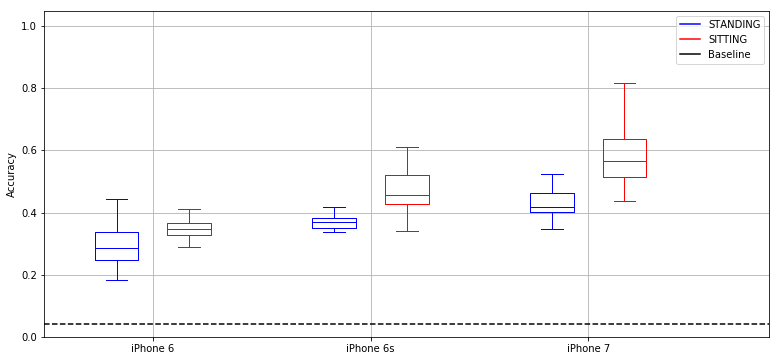
\includegraphics[width=1\textwidth]{results/standing-vs-sitting-5x4.png}
  \caption{The figure shows the tap inference accuracies for the 5x4 grid of the 10-fold cross-validation.} \label{fig:bodypos5x4}
\end{figure}

\section{Cross User Experiment}
In order to determine if it is possible to train a classifier with data from a set of users to infer taps from people not involved in the training phase, a cross user experiment was performed. Here, a SVM classifier was trained for each subject with laboratory data from 4 randomly selected subjects sharing the same device. The subject's field data was then tested on the classifier and the accuracy was measured.

For each subject, the accuracy results for the 5x4 grid are displayed in in the bar chart \ref{fig:cross_user_exp}. It can be seen that for user 86 the prediction accuracy was at minimum value of 0.09 whereas for user 87 the overall maximal value of 0.34 could be measured. The mean score measured was 0.25.

% In this experiment a classifier has been trained for each subject on laboratory data from 4 randomly selected subjects sharing the same device. In order to determine how the tap inference would behave in the field on a classifier trained on laboratory data, each subject's field data is tested on the classifier.

\begin{figure}[h!]
  \centering
  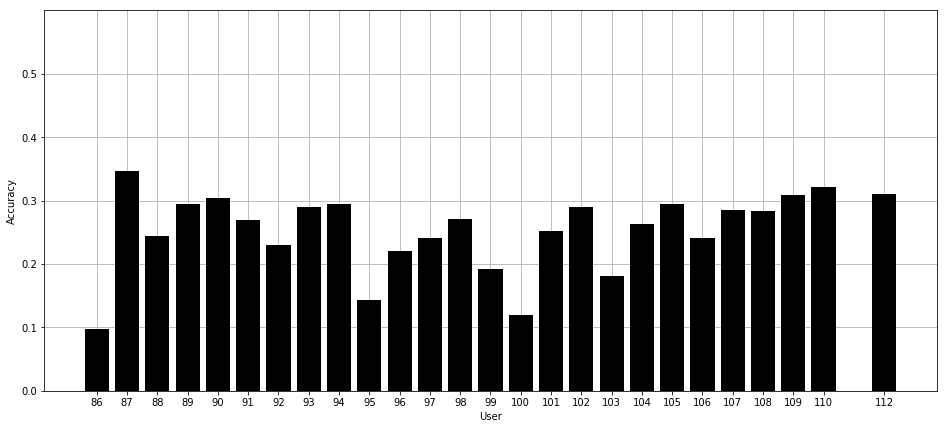
\includegraphics[width=1\textwidth]{results/classifer_lab_field.png}
  \caption{Results of the cross user experiment on the 5x4 grid.} \label{fig:cross_user_exp}
\end{figure}


